\documentclass[3p,final,twocolumn]{elsarticle}
%\documentclass[3p,times,twocolumn]{elsarticle}

\usepackage{lineno}

 \usepackage[flushleft]{threeparttable}
 \usepackage{tablefootnote}

\usepackage{graphicx}% Include figure files
\usepackage{dcolumn}% Align table columns on decimal point
\usepackage{amsmath}
\usepackage{amssymb}
\usepackage{epstopdf}
\usepackage{multirow}
\usepackage{color}
%\usepackage{longtable}
\usepackage{braket}
%\usepackage{hepparticles} % particle names
%\usepackage{hepnames} % shortcuts for lots of particle names
\usepackage[alsoload=hep]{siunitx}
\sisetup{ per-mode=symbol}
\usepackage{hyperref}
%\let\oldbibitem\bibitem
%\def\bibitem{\vfill\oldbibitem}

\usepackage{subcaption}
%\captionsetup[subfigure]{labelformat = parens, labelsep = space, font = small}

\graphicspath{{figures/}}

\modulolinenumbers[5]

\journal{}
\bibliographystyle{elsarticle-num}

 %To reset corresponding author \corref. Known bug in elsevier (https://tex.stackexchange.com/questions/116515/elsarticle-frontmatter-corresponding-author)
\makeatletter
\def\@author#1{\g@addto@macro\elsauthors{\normalsize%
    \def\baselinestretch{1}%
    \upshape\authorsep#1\unskip\textsuperscript{%
      \ifx\@fnmark\@empty\else\unskip\sep\@fnmark\let\sep=,\fi
      \ifx\@corref\@empty\else\unskip\sep\@corref\let\sep=,\fi
      }%
    \def\authorsep{\unskip,\space}%
    \global\let\@fnmark\@empty
    \global\let\@corref\@empty  %% Added
    \global\let\sep\@empty}%
    \@eadauthor={#1}
}
\makeatother


%%%%%%%%%%%%%%%%%%%%%%%%%%%%%%%%%%%%%%%%%%%% 
\newcommand*{\MIT }{Massachusetts Institute of Technology, Cambridge, Massachusetts 02139, USA}
\newcommand*{\ODU}{Old Dominion University, Norfolk, Virginia 23529, USA}
\newcommand*{\JLAB}{Thomas Jefferson National Accelerator Facility, Newport News, Virginia 23606, USA}
\newcommand*{\TAU }{School of Physics and Astronomy, Tel Aviv University, Tel Aviv 69978, Israel}
\newcommand*{\Penn}{Pennsylvania State University, University Park, PA, 16802, USA}
\newcommand*{\NRC}{Nuclear Research Center Negev, Be'er Sheva 84190, Israel}
\newcommand*{\FSU}{Florida State University, Tallahassee, Florida 32306, USA}
\newcommand*{\UTFSM}{Universidad T\'{e}cnica Federico Santa Mar\'{i}a, Casilla 110-V Valpara\'{i}so, Chile}


\begin{document}


%%%%%%%%%%%%%%%%%%%%%%%%%%%%%%%%%%%%%%%%%%%%%%%%%%%%%%%%%%%%%%%%%%%%%%%%%%%%%%%%%%%%%%%%%%%%%%%%%%%
\begin{frontmatter}

\title{The CLAS12 Backward Angle Neutron Detector (BAND) }

%% Group authors per affiliation:


\author{E.P.~Segarra}
\author{F.~Hauenstein\corref{mycorrespondingauthor}}
\ead{hauenst@jlab.org}

\author{A.~Schmidt}
\author{A.~Beck}
\author{S.~May-Tal Beck}
\author{R.~Cruz-Torres}
\author{A.~Denniston}
\author{A.~Hrnjic}
\author{T.~Kutz}
\author{A.~Nambrath}
\author{J.~Pybus }
\author{O.~Hen}
\address{\MIT}

\author{K.~Pryce\fnref{orsay}}
\author{C.~Fogler}
\author{T.~Hartlove}
\author{L.B.~Weinstein}
\address{\ODU}
%ADD current address for Kitty (Orsay)
\author{I.~Vega}
\author{M.~Mu\~nos}
\author{H.~Hakobyan}
\author{W.~Brooks}
\address{\UTFSM}
\author{E.~Piasetzky}
\author{E.~Cohen}
\author{M.~Duer}
\address{\TAU}
\author{I.~Korover}
\address{\NRC}
\author{P.~Eugenio}
\address{\FSU}

\cortext[mycorrespondingauthor]{Corresponding Author}
\fntext[orsay]{Current address: Institut de Physique Nucl\'{e}aire, IN2P3-CNRS, F-91406 Orsay, France}
%%%%%%%%%%%%%%%%%%%%%%%%%%%%%%%%%%%%%%%%%%%%%%%%%%%%%%%%%%%%%%%%%%%%%%%%%%%%%%%%%%%%%%%%%%%%%%%%%%%
\date{\today}
%\ead[]{}
\begin{abstract}
 The Backward Angle Neutron Detector (BAND) of CLAS12 detects neutrons
  emitted at backward angles of $155$\si{\degree} to $175$\si{\degree}
  and momenta between $0.25$ and $0.6$ \si{\GeV/\clight}. It is
  positioned 3-\si{\meter} upstream of the target and consists of $18$
  rows and $5$ layers of $7.2$ \si{\centi\meter} by $7.2$
  \si{\centi\meter} scintillator bars with PMT readout on both ends to
  measure time and energy deposition in the scintillator
  layers. Between the target and BAND there is a 2-\si{\centi\meter}
  thick lead wall followed by a 2-\si{\centi\meter} veto layer to
  suppress gammas and reject charged particles. The momentum
  reconstruction resolution is $\delta p/p < 1.5$\% in the design
  momentum range.
\end{abstract}

\begin{keyword}
CLAS12; time of flight; plastic scintillator; fast neutrons
\end{keyword}
\end{frontmatter}

%%%%%%%%%%%%%%%%%%%%%%%%%%%%%%%%%%%%%%%%%%%%%%%%%%%%%%%%%%%%%%%%%%%%%%%%%%%%%%%%%%%%%%%%%%%%%%%%%%%
\linenumbers


\setcounter{footnote}{0}
\renewcommand{\thefootnote}{\alph{footnote}}
\section{Introduction}


CLAS12 (12-GeV CEBAF Large Acceptance
Spectrometer)~\cite{Burkert:2020akg} in Hall B of the Thomas Jefferson
National Accelerator Facility (JLab) is a multi-purpose spectrometer
used to detect charged and neutral particles emitted in high-energy
electron scattering reactions.  Tagged deep inelastic scattering studies
in electron-deuteron interactions require the detection of backward
angle recoil
neutrons with momenta above \SI{250}{\mega\eVperc}.
This is achieved by a combination of the Central Neutron Detector
(CND)~\cite{Chatagnon:2020lwt} and the Backward Angle Neutron Detector
(BAND). The CND covers angles from $40$\si{\degree} to
$120$\si{\degree} while BAND covers from $155$\si{\degree} to
$175$\si{\degree}.

This paper describes BAND. BAND was designed to measure neutrons with
momenta of $0.25 - 0.6$ \si{\GeV/\clight} with a detection efficiency
of $35$\% and momentum reconstruction resolution better than
$1.5\%$. It is based on scintillator bars with PMT readout.  BAND was
installed in January 2019 and has taken data in coincidence with
CLAS12. Fig.~\ref{fig:clas12band} shows a drawing of BAND located
upstream of CLAS12 in Hall B.


\begin{figure}[t!]
	\centering
	\includegraphics[width=0.49\textwidth]{BandInClas.png}
        \caption{CLAS12 and BAND in Hall B at Jefferson Lab. The
          electron beam is incident from the right side. BAND is
          marked in red. The overall detector system is roughly 20
          \si{\meter} in scale along the beam axis. }
		\label{fig:clas12band}
\end{figure}

Chapter 2 presents the required time resolution, efficiency and
geometry, the resulting design and layout, the selection of detector
components, and results from comparative measurements of different
PMTs and magnetic shields. Chapter 3 presents the performance of the
detector after its installation in Hall B. It describes cosmic-ray and
laser calibrations ~\cite{band-laser} as well as the measured
time-of-flight (ToF) resolutions and neutron-photon separation from
$10.6$-\si{\GeV} electron-deuteron data. Chapter 4 summarizing the
results.



%%%%%%%%%%%%%%%%%%%%%%%%%%%%%%%%%%%%%%%%%%%%%%%%%%%%%%%%%%%%%%%%%%%%%%%%%%%%%%%%%%%%%%%%%%%%%%%%%%%

\section{Design of the backward angle neutron detector}
The major considerations for the BAND design were the constraints on
geometry and areal coverage in Hall B, the time-of-flight resolution
required and, neutral particle identification.  To achieve the physics
of interest with neutrons in BAND~\cite{band-proposal}, ToF
resolutions below $300$ \si{\pico\second} at an energy deposition
threshold of $\sim 3$ MeVee (MeV electron equivalent) are required. Neutral-particles are
identified by using a thin $1$-\si{\centi\meter} veto layer for
charged-particle identification between the target and the first
active layer of BAND. Photons are suppressed by a 20-\si{\milli\meter}
thick Lead wall placed downstream of the veto layer. Neutron-photon
discrimination is achieved via ToF relative to the electron scattering
time measured by CLAS12. Off-time random neutron and photon
contamination is reduced by optimizing the energy-deposition cuts.

The next subsections describe the details of the individual BAND components,
including results from bench measurements. In addition,
this section also includes information on the lead shielding, laser
calibration system, readout electronics and the high voltage system as
well as pictures from the final assembly of the detector.


\subsection{Geometry}
%% ALSO TABLES FOR GEMOETRY< PMTS ADN SCINTILLATOR IN THIS CHAPTER. PART OF IT IN GEOMETRY
%%ALSO LIGHTGUIDES!!
%%GEMOETRY CONSTRAINTS: LENGTH BY SIZE, CROSS SECTION BY COSTS
\begin{figure}[tb]
	\centering
		\includegraphics[width=0.40\textwidth]{FULL_CONTEXT_STUDIE_3.png}
		\vspace{0.5cm}
	    \caption{BAND and its close surroundings: the
                  cyrotarget and beam line components (cyan),  BAND
                  (red), the central detector region of CLAS12
                  (blue), the space fram (black), and the central detector support cart (gray). The beam is coming from the left side. The
                  target is located at the center of the CLAS12 central detector}
		\label{fig:bandtarget}
		
\end{figure}

The geometry of the BAND was constrained by the requirement to detect
backward angle neutrons and by the physical constraints in the hall (see 
Fig. \ref{fig:bandtarget}). BAND had to be positioned between the
target support and the central detector region of CLAS12 to reduce
scattering of neutrons on material in their flight path. Furthermore,
BAND had to be placed on the support cart for the central tracking
detectors of CLAS12 and lowered
onto the cart from an existing opening in the floor above it (black in Fig. \ref{fig:bandtarget}).

These requirement constrained BAND to fit within a
box 3-\si{\meter} wide, 1.5-\si{\meter} high, and 1-\si{\meter}
deep, with a hole in the middle for the beam pipe.

To maximize the active detector volume within these constraints, we
chose to use rectangular scintillator bars layered perpendicular to
the beam direction ($z$), see Fig.~\ref{fig:design}.  The cross
section of each scintillator bar determines our position granularity
in $y,z$ (vertical and longitudinal directions relative to the beam
pipe), which is comparable to our time-resolution-dependent position
resolution along the bar. Given our time-resolution specification of
$300$ \si{\pico\second} (discussed below), $7.2$
\si{\centi\meter} by $7.2$ \si{\centi\meter} scintillator bars were
chosen to optimize fiducial volume, granularity, and cost.


\begin{figure}[tb]
	\centering
	%\includegraphics[width=0.48\textwidth]{MAIN_DETECTOR_COLORED_2.png}
	%	\includegraphics[width=0.48\textwidth]{VETO_DETECTOR_COLORED_2.png}
			\includegraphics[width=0.48\textwidth]{band-schematic.pdf}
            \caption{BAND design of bars in the main
                   detector and the veto layer. The 164-\si{\centi\meter} long bars are shown in
                          red, the 202-\si{\centi\meter} bars in white
                          and the short, 51-\si{\centi\meter} bars in cyan. The position of
                          the PMTs for each bar is also shown. The beam direction corresponds to the $z$-axis.   }
		\label{fig:design}
\end{figure}

The active detector area consists of 116 scintillator bars, arranged
in 5 layers with 18 vertically stacked bars. The arrangement of the
bars is shown in Fig. \ref{fig:design}. The bottom three rows each have only
four layers due to obstructions from the cart below BAND.

Three different bar lengths are used: 15 164-\si{\centi\meter} bars, 43 202-\si{\centi\meter} bars, and 58 
51-\si{\centi\meter}  bars. The shorter bars were used in the vicinity of
the beam pipe. All bars have light guides attached to both sides which
are readout by either Hamamatsu R7724 \cite{pmtR7724} or Electron
Tubes (ET) 9214KB \cite{pmt9214} 2-inch PMTs.

The veto layer, which is installed on the downstream face of BAND
(i.e., between BAND and the target),
consists of 24 scintillator bars with a cross section of $2$
\si{\centi\meter} by $7.2$ \si{\centi\meter}. The veto bars have the
same lengths as the corresponding BAND bars such that the whole
downstream surface is covered by the veto, see
Fig. \ref{fig:design}. Each veto bar is only read-out on one side by a
single ET 9954KB \cite{pmt9954} 2-in PMT.

Each bar has an assigned sector and layer number. The layer number
corresponds to the position along the beam line starting
from upstream (1) to downstream (5) for the active area and (6) for
the veto bars. The sector numbering follows from top to bottom. The
middle-long bars in the top three rows make up sector 1 (red in
Fig.~\ref{fig:design}). Sectors 2 and 5 consists of the 202-cm long bars above
(seven rows total) and below (two rows total) the short bars,
respectively (white in Fig.~\ref{fig:design}). The short bars to the
left of the beam hole are sector 3, while the ones on the right side
are sector 4 (cyan in Fig.~\ref{fig:design}).
Table~\ref{tab:geometry} summarizes the geometry parameters and PMTs
for each sector and layer.


%NOT PERFECT PHI SYMMETRY BUT NOT IMPORTANT FOR BAND PHYSICS
\begin{table}[t]
\caption{Parameters for bars and PMTs for the different BAND sectors and layers.}
\centering
\begin{tabular} {l  l  m{4em}} \hline
 &  Dimensions ($w\times h$) & PMT \\ \hline\hline
\multicolumn{3}{l} {Sector 1,  $L = 164~\si{\centi\meter}$} \\ \hline
Layer $1 - 5$  & 7.2$\times$7.2 \si{\centi\meter\squared} & R7724  \\
Layer 6  & 2$\times$7.2 \si{\centi\meter\squared} & 9954KB  \\
\hline
\multicolumn{3}{l} {Sector 2, $L = 202~\si{\centi\meter}$} \\ \hline
Layer $1 - 5$  & 7.2$\times$7.2 \si{\centi\meter\squared} & R7724  \\
Layer 6  & 2$\times$7.2 \si{\centi\meter\squared} & 9954KB  \\
\hline
\multicolumn{3}{l} {Sector 3 / 4, $L = 51~\si{\centi\meter}$} \\ \hline
Layer $1 - 4$  & \multirow{2}{*}{7.2$\times$7.2 \si{\centi\meter\squared}} & 9214KB \\
Layer 5 & & R7724 \\
Layer 6  & 2$\times$7.2 \si{\centi\meter\squared} & 9954KB  \\
\hline
\multicolumn{3}{l} {Sector 5, $L = 202~\si{\centi\meter}$ } \\ \hline
Layer $1 - 4$\tablefootnote{Layer 5 is missing due to obstructions from below}  & 7.2$\times$7.2 \si{\centi\meter\squared} & R7724  \\
Layer 6  & 2$\times$7.2 \si{\centi\meter\squared} & 9954KB  \\
\hline
\end{tabular}
\label{tab:geometry}
\end{table}
%%%%%%%%%%%%%%%%%%%%%%%%%%%%%%%%%%%%%%%%%%%%%%%%%%%%%%%%%

\subsection{Components}
The timing resolution of the scintillator bars is affected by many
factors, and each component was optimized considering both cost and
 design constraints.
We selected Bicron BC-408 \cite{scint-mat-ref} scintillant for its
light output, time
response and attenuation length. The bulk attenuation length of 380
\si{\centi\meter} is much longer than the bars, ensuring sufficient
photon statistics at both ends. To enhance reflectivity, we wrapped
each bar with 3M Enhanced Specular Reflector foils~\cite{3MESR}. 
We bench-tested different PMT and magnetic shielding options.
% Tests were performed varying the scintillant, reflective wrapping, photo-multipler tube (PMT), and optical-coupling-method of the scintillators to light-guides to PMTs to select the optimal combination

\begin{figure}[th!]
	\centering
	%	\includegraphics[width=0.48\textwidth]{phys_setup.png} \\
		\includegraphics[width=0.48\textwidth]{setup-diagram.pdf} \\
		\includegraphics[width=0.48\textwidth]{electr_setup.png}
	\caption{Schematic of the bench test setup (top) and its
          read-out system (bottom) to measure PMT time resolutions. }
	\label{fig:test_stand_setup}
\end{figure}

\subsubsection{Bench Measurements}
Bench measurements were used to guide the PMT and magnetic shielding
selection.  A diagram of our test setup and electronics is shown in
Fig. \ref{fig:test_stand_setup}, featuring a coincidence setup between
a ``test'' scintillator bar and a ``reference'' scintillator bar.  Each
bar has two PMTs coupled to its ends; the test bar has the PMTs whose
time resolution we wish to study.  Both bars are wrapped in an optical
reflector, and placed in a dark-box.  The reference bar was kept fixed
during all measurements.  We tested five different 2-in PMTs (see
\cite{hamapmts} and \cite{pmt9214}), assembled on 200 to 250
\si{\centi\meter} long bars.

The signal for our measurement is produced by a $^{60}$Co source which
is placed between the two bars.  The $^{60}$Co source produced two
$\gamma$ rays with energies of 1.17 and 1.3 \si{\mega\electronvolt}.
The two $\gamma$-rays were collimated by two lead bricks to ensure
they each hit a specific location along each bar, allowing us to study individual
PMT time resolution and measured energy as a function of hit location.

\begin{table}[t!]
	\caption{Bench test configurations. Length refers to the length of the scintillator bar.  $\sigma$ is the time
          resolution for $2$ \si{\mega\electronvolt} central-equivalent energy deposit in the middle of the bar
          extrapolated from data.  The 9214KB PMT \cite{pmt9214} is manufactured by ET-Enterprises and the other PMTs are manufactured by Hamamatsu \cite{hamapmts}.}
    \centering
	\begin{tabular}{ m{5em}   m{3em}   m{3em} }
		\hline
			PMT & Length (cm) & $\sigma$ (\si{\pico\second})\\
		\hline\hline
%			R7724 & ESR &   200 & 150	\\
			R7724 &  200 &  240		\\
			R7724-100 & 250 & 212 		\\
			R13089 & 250 & 213			\\			
			R13435 & 200 & 308 			\\		
			9214KB & 200 & 257			\\
%			ET-9214KB &  ESR & 50 & 150				\\
		\hline
	\end{tabular}
	\label{tab:tests}
\end{table}
% FOR NIM ADD 3M Enhanced Specular Reflector \cite{3MESR}) RESULTS

We combined measurements with different $^{60}$Co
source locations by using the measured attenuation in the bar to convert
the energy measured by the PMT to the ``center-equivalent energy
deposit'', the energy that would have been deposited at the center of
the bar to give the same measured energy.  For example, by placing the
source close to one PMT we can achieve a center-equivalent energy
deposit significantly greater than the 1 \si{\mega\electronvolt} $^{60}$Co Compton edge.
% To combine measurements with different $^{60}$Co source locations, we
% used the center-equivalent energy deposit, determined by taking into
% account the attenuation length, and normalized the PMT response to the
% $^{60}$Co placed at the center of the bar.
Fig.~\ref{fig:test_stand_posdep} shows the PMT time resolution as a
function of  center-equivalent energy deposited for different source placements. Since
the individual data sets are consistent within error bars, we combined
the measurements to cover a center-equivalent energy deposition range
up to 1.8 \si{\mega\electronvolt}.

\begin{figure}[tb]
	\centering
		\includegraphics[width=0.48\textwidth]{pos-dep.pdf}
		\caption{PMT time resolution as a function of
                  center-equivalent energy deposit for different
                  placements of the $^{60}$Co source along the bar for
                  Hamamatsu R13089 PMT. The labels indicate the
                  distance of the source to the PMT. }
	\label{fig:test_stand_posdep}
\end{figure}

Fig. \ref{fig:test_stand_results} shows the measured single-PMT time
resolution for the different test configurations.  The lines indicate fits
to data extrapolated beyond 1.8 \si{\mega\electronvolt}.  
All PMTs except the R13435 met the timing-resolution design specifcation of 300 \si{\pico\s} at 2
\si{\mega\electronvolt} energy deposition (see 
Table~\ref{tab:tests}).  To reduce costs, we chose a combination of
Hamamatsu R7724 \cite{pmtR7724} and Electron Tube 9214KB
\cite{pmt9214} PMTs for BAND. For the veto layer, we used 
available Electron Tube 9954KB PMTs. See Table \ref{tab:pmts} for
details of the PMTs.

\begin{figure}[tb]
	\centering
		\includegraphics[width=0.48\textwidth]{all-lines-somedata.pdf}
		\caption{Single-PMT time resolution as a function of center-equivalent energy deposit for the five PMTs
                  tested. The lines are fits to data (only the blue  and yellow data points are shown). At 2
                  \si{\mega\electronvolt} energy deposition all PMTs except R13435 achieve a time resolution below 300 \si{\pico\s}.}
          	\label{fig:test_stand_results}
\end{figure}

\begin{figure}[tb]
	\centering
		\includegraphics[width=0.48\textwidth]{resolution-laser-scan.pdf}
		\caption{Time resolution as a function of center energy deposit for one bar with R7724 PMTs using the
                  BAND laser system after installation. The energy deposition is the geometric mean of both PMTs at the
                  end of the bar. The deposition is in the center of the bar due to the installation of the fiber there. }
         \label{fig:resolution-laser}
\end{figure}

After BAND was assembled, we measured the time resolution as a function
of energy deposit in the center of the bar using the laser calibration
system (see Sec. \ref{sec:laserystem} and \cite{band-laser}).
Fig. \ref{fig:resolution-laser} shows the results for a representative
long BAND bar with R7724 PMTs.  The resolution is better than 250
\si{\pico\s} from 1 to 7 \si{\mega\electronvolt} central energy
deposition, indicating the good performance of the bars and PMTs. The
laser results are not fully comparable with the source results since
the energy deposition refers here to the geometric mean of both PMTs
and the time resolution refers to the combined two-PMTs of the bar and
not to a single PMT.

%\subsubsection{PMTs, Voltage Dividers and Light Guides}

\begin{table*}[tbh]
\caption{Properties of the PMTs used in BAND. }
\centering
\begin{tabular} { l  l  l l } \hline
 &  R7724 \cite{pmtR7724} & 9214KB \cite{pmt9214}& 9954KB \cite{pmt9954} \\ \hline\hline
Company                                  & Hamamatsu       & ET           & ET \\
Diameter                                           & 2~in                         & 2~in                        & 2~in \\ 
Dynode stages                                  & 10                           & 12                              & 12 \\
Spectral response                            & 300 $\to$ 650~nm & 290 $\to$ 630~nm & 290 $\to$ 680~nm \\ 
Max. wavelength emission               & 420~nm & 350~nm & 380~nm \\ 
Quantum eff. @ $\lambda_{max}$   & 26\% & 30\% & 28\% \\ 
Gain                                                    & 3.3$\times$10$^6$ & 3.0$\times$10$^7$ & 1.8$\times$10$^7$ \\ 
Max. anode current rating               & 200~$\mu$A & 100~$\mu$A & 100~$\mu$A \\ 
Anode dark current                         & 6~nA  & 4~nA & 8~nA \\ 
Anode pulse rise time                      & 2.1~ns & 2.0 ns & 2.0 ns \\ 
Electron transit time                        & 29 ns & 45 ns & 41 ns \\
\hline
\end{tabular}
\label{tab:pmts}
\end{table*}

\subsubsection{Light Guides}

The light guides design was constrained by the available space and the
sizes of the scintillator bars and PMTs. CAD drawings of the light guides for the main detector and the veto bars are shown in Fig. \ref{fig:lightguides}. They are 9 \si{\centi\meter} long. Each light guide has a 5 \si{\centi\meter} long tube end with 2-in diameter connected to the PMTs to allow for a cover of an area in front of the photocathode with magnetic shields (see next section). The other end of the light guide matches the cross section of a bar. It is glued to the bar with a DYMAX UV curing glue \cite{uvglue} and to the PMT with a RTV615 soft glue \cite{softglue}. All light guides were designed by UTFSM in Chile and manufactured by Florida State University.  
\begin{figure}[tb]
	\centering
	\includegraphics[width=0.23\textwidth]{bar_lg.png}
		\includegraphics[width=0.18\textwidth]{veto_lg.png}
	\caption{CAD drawing of the light guides for the main detector (left) and the veto bars (right). The top parts are connected to the 2-in PMTs while the lower parts are connected to the bars.}
	\label{fig:lightguides}
\end{figure}

\subsubsection{PMT Magnetic shielding}
The fringe-field of the CLAS12 solenoid magnet
\cite{Fair:2020yfx} was between 20 and 120 \si{\gauss} at the location of
BAND so that all PMTs required magnetic shielding. The transverse
field (perpendicular to the axis of the PMT) in the PMT region ranged from 10 to
  110 \si{\gauss} and the longitudinal field ranged from 10 to 50 \si{\gauss}.

  A dedicated test stand was used to examine different thicknesses of
  passive magnetic shielding.  We constructed two 56-turn Helmholtz
  coils with a radius of 0.5 \si{\meter}, separated by 1 \si{\meter}. A
  prototype detector consisting of a 2 \si{\centi\meter} thick, 5
  \si{\centi\meter} diameter scintillator disc, coupled to two
  7-\si{\centi\meter} long, 5-\si{\centi\meter} diameter cylindrical
  acrylic light guides and two PMTs. The detector was
  light-proofed with Tedlar and stabilized on a simple plastic stand
  at the center of the Helmholtz coils.

  As a baseline, we measured the zero-magnetic-field 
event rates, time difference between the left and right PMT signals,
and the left and right PMT energy peak locations for $^{90}$Sr and
  $^{137}$Cs sources at two locations (at 0 and 5 \si{\centi\meter} from the scintillant) and  at nominal
  PMT operating voltage and no shielding.  We then measured the same quantities with different
  shielding configurations at different longitudinal and transverse
  magnetic fields up to 80 \si{\gauss} (limited by heat dissipation in the
  Helmholtz coils).

  We tested $\mu$-metal shielding with  thicknesses of 0.9, 1.5, 1.8,
  2.4 and 3 \si{\milli\meter}, as well as two soft-iron pipes. The magnetic field, amount of detector covered by the
  shielding, the thickness of the shielding, and the angle of the detector to the field were
  all varied.
  
In Fig. \ref{fig:shielding_results}, the event rate as a function of magnetic field strength is shown for different  thick $\mu$-metal shields and a reference measurement without any shield. These results are from a $^{90}$Sr source, a longitudinal field setting and placing the shield to cover 5 \si{\centi\meter} beyond the photocathode. 
The longitudinal magnetic field degraded the PMT performance
the most.  We found that the 1.5-\si{\milli\meter} $\mu$-metal shield was not
sufficient, but that the 1.8-\si{\milli\meter} $\mu$-metal shield maintained PMT
performance up to 80 G.  The soft-iron pipes performed worse than the
1.5-\si{\milli\meter} $\mu$-metal (not shown in Fig. \ref{fig:shielding_results}. The magnetic shields performed best when they
extended 5 \si{\centi\meter} (one diameter) beyond the PMT photocathode.  In order to
be conservative, we selected 2.6-mm thick $\mu$-metal shields.

\begin{figure}[tb]
	\centering
			\includegraphics[width=0.47\textwidth]{shielding_results.pdf}
	\caption{Magnet shielding test results with a $^{90}$Sr source, a longitudinal field and shields placed covering 5 \si{\centi\meter} beyond the PMT photocathode. Event rate with increasing field without any shielding are shown in green. The results with various $\mu$-metal shields are indicated by the other colors with their thickness written in the plot. }
	\label{fig:shielding_results}
\end{figure}


\subsubsection{PMT and bar quality test measurements}
Before the final assembly of BAND (see Section \ref{sec:assembly}), all PMTs and bars have been tested on the bench for quality. These measurements were conducted with a LED pulser.
For each bar the attenuation length was measured by moving the LED pulser along the bar. This has been done without a wrapping material around the bar in a light tight black-box. The bars with the worst attenuation length were selected as back-up bars.

The test setup for each PMT had a 6.4 \si{\centi\meter} long scintillator disc attached between the LED and the PMT. We measured gains and time resolutions for each PMT. The PMTs were matched in pairs according to their gains and each pair was installed on a bar.


\subsection{Lead shielding}
To minimize background from backward going photons, we installed a
lead wall on the downstream face of BAND (between the CLAS12 target
and BAND). This lead wall consists of individual 20-\si{\milli\meter}
thick blocks stacked in front of the veto layer. Each block is covered
on both sides with an Aluminium layer to simplify handling. The
lead wall can be seen on the final assembly pictures shown in
Fig. \ref{fig:band_downstream}.


\subsection{Laser Calibration system}
\label{sec:laserystem}
We implemented a UV laser system to calibrate BAND and monitor its
performance during data-taking. The design and performance of the
system is fully described in Ref. \cite{band-laser}. 

The main component of the system is a picosecond pulsed diode laser (Teem Photonics STV-01E-140, \cite{teem_laser}) with a wavelength of 355 \si{\nano\meter}. The laser can be triggered externally between $10-2000$ \si{\hertz}. The light is only transported within fibers. Further components of the system are a mode scrambler, a 90:10 splitter whose outputs are connected to a reference photodiode (10\% output) and a variable optic attenuator \cite{attenuator} (90\% output). The attenuator allows to vary the pulse intensity sent to the detector. It is connected to a custom SQS Vl\'aknov\'a Optika 1$\times$400 splitter which distributes the light to every bar of BAND. 

Each bar has an optical fiber glued to its center with UV-cure glue (see
Fig. \ref{fig:pic-fiberonbar}). We used an exposed fiber for the fiber-scintillant connection since it was a stable, reliable and easy option. The other end of the fiber is connected to the splitter through a patch panel attached to the BAND frame. 

The photodiode provides reference time for the laser system. The output
signal of the photodiode is inverted and shaped before it is sent to
the BAND read-out system. The signal is then digitized by the same ADCs and
TDCs which are used for the PMT signals.

% Windows for easy access were kept inthe wrapping foils around the bar. The windows were stacked with
% different alignments to reduce light leaks. After the installation of the fiber, the bar was intensively tested for light-leaks.
\begin{figure}[tb]
	\centering
		\includegraphics[width=0.40\textwidth]{pic-fiberonbar.pdf}
	\caption{Connection of a fiber to bar after UV-cure gluing. The fiber is positioned in the center of the bar and is covered by both layers of wrapping material, ESR \cite{3MESR} and Tedlar foil \cite{tedlarfoil}.}
	\label{fig:pic-fiberonbar}
\end{figure}



%%% ----------------- Electronics subsection
\subsection{Electronics and DAQ}
%TODO SOME UPDATES ON THE FADC SIGNALING, HV CONTROL, TABLE WITH TDC AND ADC PARAMETERS
%The threshold for the discriminators similar for disc and FADC. The pulse shape from the flash-ADCs are recorded for every PMT crossing a threshold value allow to record the signal amplitude and integral. The integral window can be adjusted offline in the pulse fitting algorithm.
%For the data shown here is was set to 80ns = 20 samples
%\begin{table*}[htbp]
%\caption{Key performance specifications of the CAEN V1190A TDCs and the JLab FADC250 flash ADCs.}
%\centering
%\begin{tabular}{c|c} \hline
%TDC Specs (1190A) & ADC Specs \\ \hline
%No. Channels: 128             & 16               \\ 
%RMS resolution 100~ps          & Sampling 250 MHz \\
%Resolution: 19~bit                  & Resolution: 12-bit \\ 
%Inter-channel isolation $\le$ 3 LSB & Clock jitter 350~fs \\ 
%Double-hit resolution 5~ns          & Data memory 8~$\mu$s \\  
%Full-scale range 52~$\mu$s          & Trigger/Data latency 8~$\mu$s / 32~ns \\
%\end{tabular}
%\label{table:tdcadc-specs}
%\end{table*}
\begin{figure}[tb]
	\centering
	\includegraphics[width=0.48\textwidth]{electronics-diag.pdf}
	\caption{Electronic schematic of the BAND read-out. Every PMT signal is split and ADC and TDC information are obtained. Additional outputs of the discriminators are used to create single bar and cosmic-laser triggers from BAND.}
	\label{fig:electronic-diag}
\end{figure}

In the experiment, the high voltages for each PMT are provided by a multi-channel CAEN SYS4527 mainframe with eleven A1535SN cards with 24 channel each \cite{caen-hvframe,caen-hvcard}.

A schematic drawing of the read-out electronics and its components is
shown in Fig. \ref{fig:electronic-diag}. The signal of each PMT is
split to an ADC and TDC readout independently.  The signal splitters
are custom made and have been used in previous experiments at
Jefferson Lab.  From the splitter one signal is sent to a 250
\si{\mega\hertz} sampling flash-ADCs \cite{fadc-manual} while the
other signal is sent to discriminators.  The discriminated time signal
goes to a TDC (CAEN VX1190A \cite{caen-tdc}) with 100 ps resolution
per channel.

%The threshold for the d The pulse shape from the flash-ADCs are recorded for every PMT crossing a threshold value allow to record the signal amplitude and integral. The integral window can be adjusted 

In total, the system consists of 16 flash-ADCs in one VXS crate, 16
discriminators and two TDCs in a VME crate and 16 splitters.
A trigger signal distribution card for the flash-ADCs and
trigger interface boards are installed in the crates. All components
are part of the standard CLAS12 electronics \cite{clas12-daq, clas12-trigger}.

The detector is read-out either by a trigger from the main CLAS12
trigger system \cite{clas12-trigger} or by stand-alone BAND detector
triggers used for tests and calibrations with cosmic rays, radioactive
sources and the laser system. The stand-alone triggers are implemented
by a programmble CAEN V1495 logic board \cite{caen-logicboard}. They
consist of a single bar trigger for source measurements and a
coincidence bar trigger for cosmics and laser measurements. The
coincidence trigger is also fed to the central CLAS12 trigger system
to allow monitoring of the detector by recording laser data during
real data taking. This special trigger rate is usually about 10
\si{\hertz}, compared to the $\approx 15-20\,\si{\kilo\hertz}$ trigger
rate from electron interactions in the target.




%%% ----------------- Assembly subsection
\subsection{Final Assembly}
\label{sec:assembly}
\begin{figure*}[tb]
	\centering
	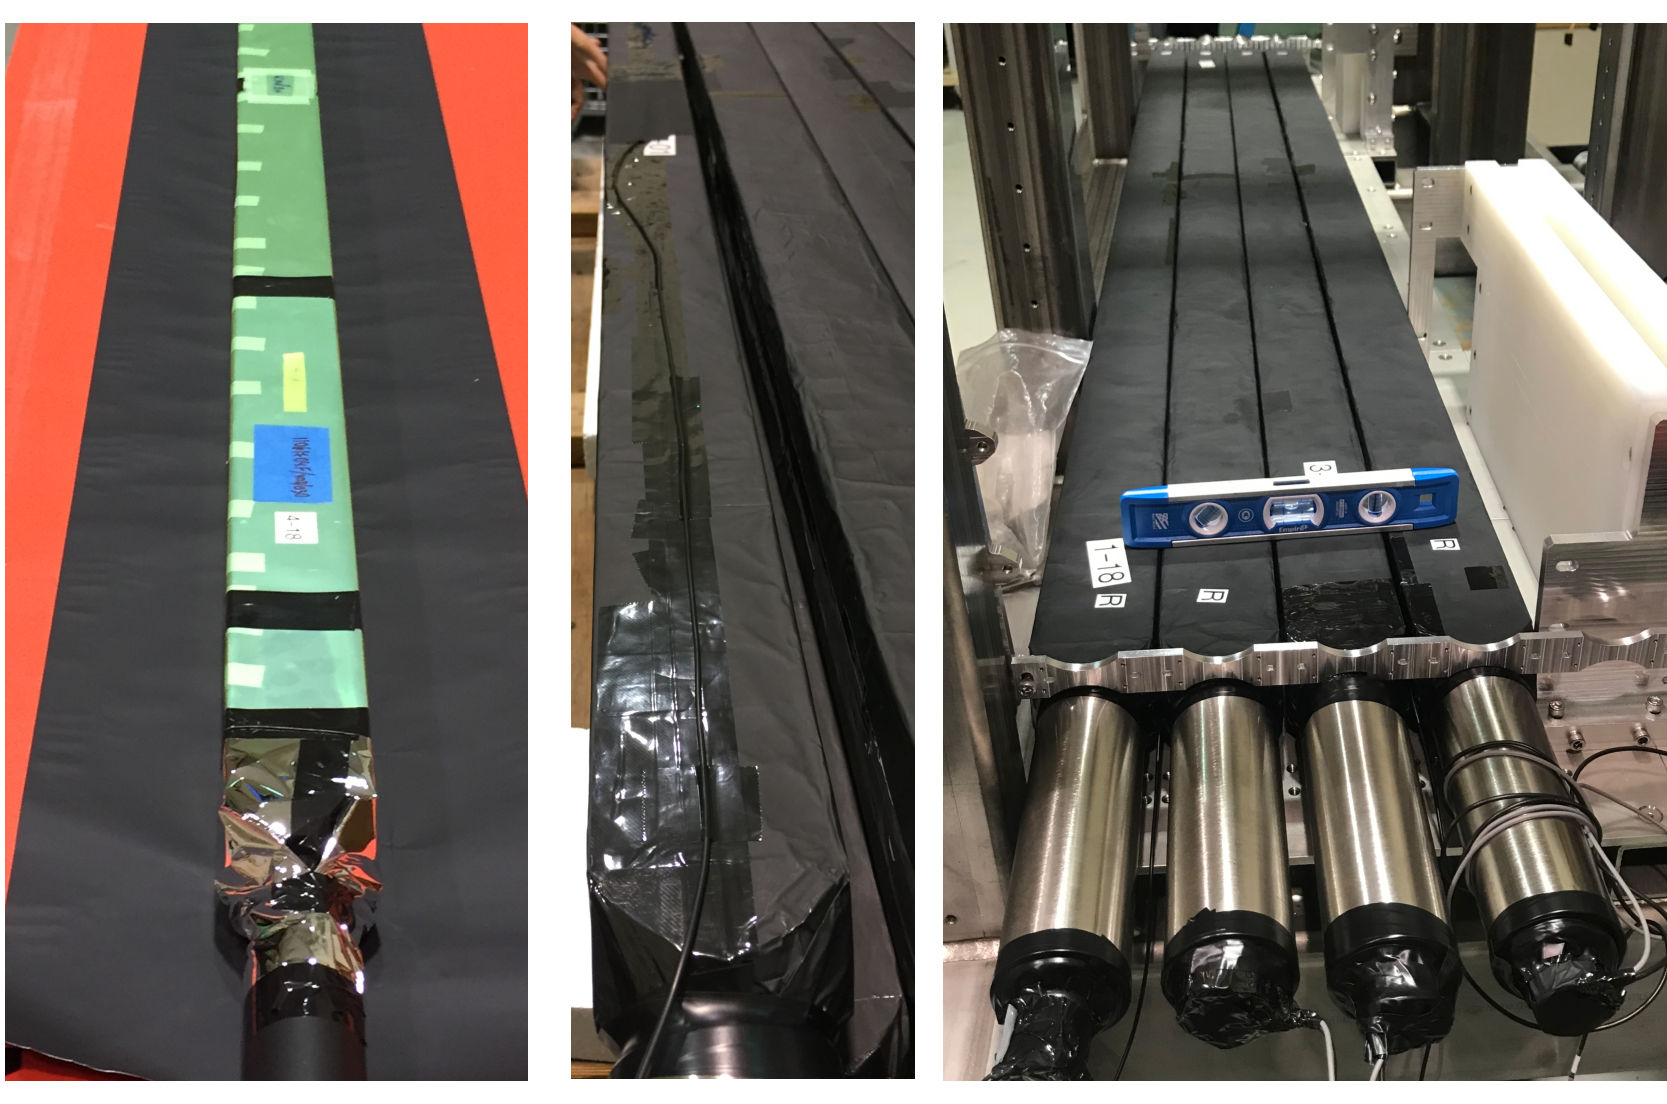
\includegraphics[width=0.48\textwidth , height=0.40\textwidth]{pic-construction1.pdf}
	\includegraphics[width=0.40\textwidth , height=0.40\textwidth]{pic-construction2.pdf}
				\caption{BAND construction. From ESR \cite{3MESR} wrapped bars (left) to assembled detector (right). The intermediate steps show the fully wrapped bars with the optical fiber and the assembled bottom row of the detector.}
		\label{fig:barassembly}
\end{figure*}
We assembled and intensively tested each scintillator bar
separately. We equipped each scintillator with a pair of gain-matched
PMTs.  Each bar undergo the following procedure:
\begin{enumerate}
\item Select a pair of gain-matched PMTs
\item Glue the PMTs to the light guides with RTV615 soft glue \cite{softglue}.
\item Glue one light guide/PMT assembly to each end of the bar with DYMAX
  UV curing glue \cite{uvglue}.
\item Wrap the assembled scintillator with Enhanced Specular Reflector \cite{3MESR}.
\item Wrap this with black 50-$\mu$m thick Tedlar foil \cite{tedlarfoil}, leaving an openable
  window for attaching the laser-system optical fiber.
\item Search for and fix light leaks by measuring the PMT dark currents with a pico-ammeter.
\item Glue the optical fiber to the center of the bar and reseal the Tedlar foil window.
\item Install the $\mu$-metal shields on the PMTs 
\item Test for light leaks (again)
\item Install each bar in the BAND support frame
\item Connect the optical fibers and signal and HV cables to patch panels mounted on the upstream side of BAND
\item Final test for light leaks
\end{enumerate}
Fig. \ref{fig:barassembly} shows some of the steps in the assembly process,
including one bar wrapped with ESR foil, a fully wrapped bar with the
optical fiber shown, a row of four bars installed in the BAND frame,
and the fully assembled BAND seen from the upstream side with the
patch panels for HV and  signal cables and optical fibers.
%%%%%%%%%%%%%%%%%%%%%%%%%%%%%%%%%%%%%%%%%%%%%%%%%%%%%%%%%%%%%%%%%%%%%%%%%%%%%%%%%%%%%%%%%%%%%%%%%%%


After assembling the bars in the support frame, the lead wall was
installed on the downstream side of BAND. BAND was then
craned into its position on top of the central vertex tracker support
cart upstream of CLAS12. Fig. \ref{fig:band_downstream} shows a
design drawing and a picture of upstream side of BAND. 
\begin{figure*}[th]
	\centering
	\includegraphics[width=0.48\textwidth]{BAND_1-2.png} 
	\includegraphics[width=0.40\textwidth]{pic-bandinhall1.pdf}
		\caption{(left) CAD drawing of the downstream side of BAND and its frame. The lead wall is shown in cyan, the scintillators
          are in magenta, and the support frame is in black. (right) Picture of the downstream side of BAND installed in Hall B. The reflective surface in the picture are the Aluminium covers of the lead blocks.}
		\label{fig:band_downstream}
\end{figure*}

Fig. \ref{fig:bandinhall} shows the upstream side of BAND in Hall B with about 3/4 of the cables installed. All cables are connected to
electronics which is installed outside of the picture on the left side.
\begin{figure}[tb]
	\centering
	\includegraphics[width=0.48\textwidth]{pic-bandinhall2.pdf}
				\caption{BAND in Hall B. Upstream side with first set of cables installed.}
		\label{fig:bandinhall}
\end{figure}


\section{Performance}
%%% ----------------- Gain matching subsection
In this chapter, we first describe the performance of the individual scintillator bars and their calibrations. We next describe the performance
of the BAND detector as a whole, with a focus on neutron identification and efficiency.

\subsection{Individual bar performance}
\subsubsection{Gain matching}
In order to have similar response to a given energy deposit across all PMTs of BAND, each PMT's HV was optimized using cosmic rays. Cosmic
ray spectra were measured with a range of HV and then combined to produce a gain curve for each PMT. These data were
collected with a cosmic trigger which required a cosmic ray passing through a single vertical layer of BAND to select nearly-vertical
cosmic rays. This corresponds to a relatively high energy deposition of 14.2 \si{\mega\eV}. For each HV setting we fit the ADC spectrum
with a Landau distribution and an exponential background to obtain the cosmic peak position. A representative ADC spectrum is shown in
Fig. \ref{fig:adc-spectrum}.  The obtained gain curve for this PMT is shown in \ref{fig:gain-curve}. The dashed lines indicate the final HV
setting to position the cosmic peak at ADC channel 15,000, which was choosen to have sufficient range for neutrons which deposit less
energy than the cosmic rays and to avoid signal overflows in the sampling FADCs dominating above ADCs of 20,000.

Each PMT gain curve was fit with a power law with parameters $\alpha$ and $\beta$
\begin{eqnarray}
	ADC	= \alpha * \left(\frac{\mathrm{HV}}{1500}\right)^{\beta},				
		\label{eqn:gain_curve}
\end{eqnarray}
where the division by 1500 was an arbitrary normalization to improve fit convergence. The value of the fit parameters for each PMT are
shown in Fig. \ref{fig:gain}. The Hamamatsu R7724 PMTs (red) are more uniform than either of the two ET PMTs, 9954KB (green) or
9214KB (blue)\footnote{We obtained similar results when using the pulse amplitude of the ADC signal instead of the integral}. 
%This uniformity was also observed in bench measurements with sources. 
However, the cosmic ray ADC peaks are well aligned after adjusting the HV based on the obtained gain curves (see Fig. \ref{fig:hv_settings}).

\begin{figure}[th]
	\centering
		\begin{minipage}{0.48\textwidth}
			\includegraphics[width=\textwidth]{adc-fit-example.pdf}
					\subcaption{}
			\label{fig:adc-spectrum}
		\end{minipage}
		\begin{minipage}{0.47\textwidth}
			\includegraphics[width=\textwidth]{gainfit.pdf}
			\subcaption{}
		\label{fig:gain-curve}
		\end{minipage}
		\caption{Gain curve measurement. (a) Typical ADC spectrum for a representative PMT with cosmic rays
                  and the fit with a Landau distribution and an exponential background. (b) Gain curve for the same
                  PMT. The dotted lines indicate the final HV setting to set the cosmic peak to ADC channel 15000. }
\end{figure}

\begin{figure}[th]
	\centering
		\begin{minipage}{0.46\textwidth}
			\includegraphics[width=\textwidth]{gainspread.pdf}
			\subcaption{}
			\label{fig:gain}
		\end{minipage}
		\begin{minipage}{0.46\textwidth}
			\includegraphics[width=\textwidth]{gainsadcresponse.pdf}
			\subcaption{}
		\label{fig:hv_settings}
		\end{minipage}
		\caption{ (a) Gain parameters for each PMT. One sees a greater spread in the Electron Tube PMTs (green and blue) than in the Hamamatsu PMTs (red). (b) $\mathrm{ADC}_{\mathrm{cosmic peak}}$ position for each bar (vetos not shown) after gain matching. All bars are well aligned.}
\end{figure}

%%% ----------------- Energy deposit subsection
\subsubsection{Energy deposit calibration}
\label{sec:energydeposit}
\begin{figure}[tbh]
	\centering
		\includegraphics[width=0.48\textwidth]{cobaltfit.pdf}
		\caption{ADC spectrum for a $^{60}$Co placed on the center of the bar along with the fit of the Compton edge.}
	\label{fig:compton_edge}
\end{figure}

%The ADC response of each PMT is converted to \si{\mega\electronvolt} energy deposition by measuring the response to 
%radioactive sources with different photon energies and thus different Compton edges. We used $^{60}$Co
%(0.963 and 1.118 \si{\mega\electronvolt}), $^{22}$Na (0.477 \si{\mega\electronvolt}), and $^{137}$Cs
%(1.062 and 0.341 \si{\mega\electronvolt}) sources.  For each bar we used the location of the ADC peak for each
%of the Compton edges measured in the center of the bar to determine ADC channel to energy conversion.  A typical fit to the Compton edge
%is shown in Fig.~\ref{fig:compton_edge}.  The extracted Compton edges for various bars are quite similar which also shows the a good gain
%matching obtained with cosmics. The  ADC channel to MeV conversion function with a linear fit is shown in Fig. \ref{fig:mev_conversion}.

The ADC response of each PMT is converted to \si{\mega\electronvolt} energy deposition by measuring the response to 
multiple radioactive sources. The sources $^{60}$Co, $^{22}$Na, $^{137}$Cs were chosen due to the gamma rays that have 
Compton edges of $0.963$ and $1.118$, $0.477$, and, $1.062$ and $0.341$, respectively (in \si{\mega\electronvolt}). The 
response to each source was measured in the center of the bar. Using the ADC response to all sources, in combination with the 
attenuation length of the bar, the ADC response can be converted to \si{\mega\electronvolt}. These measurements were done after the detector was gain matched (see previous section)

A typical response of a PMT to  $^{60}$Co is shown in Fig.~\ref{fig:compton_edge} along with a fit of the Compton edge by a parametrization described in [ADD REF]. The extracted Compton edges for various bars are quite similar which also shows the a good gain matching obtained with cosmics. Taking into account the results from cosmic ray and  source measurement, we obtain a ADC to MeV conversion function
% with a linear fit, see Fig. \ref{fig:mev_conversion}.


%\begin{figure}[tbh]
%	\centering
%			\includegraphics[width=0.48\textwidth]{mevadc.pdf}
%	\caption{TODO UPDATE PICTURE with fit: ADC to MeV conversion fit using data from source and cosmic ray measurements.}
%	\label{fig:mev_conversion}
%\end{figure}

%%% ----------------- Time-walk subsection
\subsubsection{Time-walk calibration}
Time-walk calibrations were performed with the laser system \cite{band-laser}. The fiber optic attenuator \cite{attenuator} is used to vary
the amount of light delivered to each bar. Waveforms and times are measured as the attenuator scans from $40$ \si{\decibel} to $0$ 
\si{\decibel}. Time-walk curves and calibrations are taken per PMT. The photodiode output is used as a reference time for any calibrations 
performed with the laser system.

Dependence of a typical PMT time to pulse height is seen in Fig.~\ref{fig:time_walk} (left). To correct for time-walk, we parameterize 
this dependence on pulse height of the ADC signal, $A$, as:
\begin{eqnarray}
	\begin{split}
		t_{\mathrm{PMT}}-t_{\mathrm{photodiode}}	&= \alpha + \frac{\beta}{\sqrt{\textrm{A}}}.				
		\label{eqn:time_walk}
	\end{split}
\end{eqnarray}
The residual after time-walk correction, $t_{\mathrm{PMT}}-t_{\mathrm{photodiode}}$, is shown in Fig.~\ref{fig:time_walk} (right). At pulse heights close to threshold, the 
parameterization is not flexible enough and under-estimates the strong dependence on pulse height. However, signals with pulse 
heights this low are not of interest, as a software cut on minimum energy deposition is needed to improve signal-to-background 
which removes these pulses (discussed in Section \ref{sec:neutronidentification}).

\begin{figure*}[tbh]
	\centering
		\includegraphics[width=0.48\textwidth]{timewalkpre.pdf}
		\includegraphics[width=0.48\textwidth]{timewalkpost.pdf}
	\caption{Time-walk calibration: Typical time to pulse height spectrum for one PMT with respect to the time for the reference photodiode before time-walk correction (left) and after time-walk correction (right).}
	\label{fig:time_walk}
\end{figure*}

%%% ----------------- Effective velocity subsection
\subsubsection{Effective velocity}
The relative time delays between PMTs on the same bar, and the speed-of-light in that bar, are extracted using cosmic ray 
data after time-walk calibrations are done for each PMT. The width of the relative timing distribution between the left and 
right PMT on a given bar is used to extract the effective velocity in a bar knowing the length of the bar,
\begin{eqnarray}
	\begin{split}
		t_L - t_R 	= -\frac{2x}{v}							\\
		 -\frac{L}{v}	\leq 	t_L - t_R 	\leq \frac{L}{v},				
		 \label{eqn:eff_vel}
	\end{split}
\end{eqnarray}

and the relative time offset is given by the center of the distribution (see Fig.~\ref{fig:eff_vel} left). The obtained effective velocities for each bar are shown in Fig.~\ref{fig:eff_vel} (right) distinguished between short bars (boxes) and long bars (circles). The observed difference is due to geometrical effects from the different bar length.

\begin{figure*}[tb]
	\centering
		\includegraphics[width=0.47\textwidth]{lr-offset.pdf}
		\includegraphics[width=0.47\textwidth]{eff_vel.pdf}
	\caption{
	(Left) Typical $t_{L} - t_{R}$ time spectrum in a single bar after time-walk correction for every PMT (left). The red dotted line indicates the $LR$ offset value from 0. (Right) Obtained effective velocities for each bar. The differences in effective velocities between long bars (circles) and short bars (boxes) are due to geometrical effects from the different bar length.}
	\label{fig:eff_vel}
\end{figure*}

%%% ----------------- Attenuation length subsection
\subsubsection{Attenuation length}
The light absorption length, attenuation length, of each bar is determined after the installation since its effective value depends on the properties of the bar wrapping.
We extract the attenuation length with cosmic ray data by using the 
ADC amplitude ($A$) and time measured by both PMTs in the bar:
\begin{eqnarray}
	\begin{split}
		A_L(x) &= A_0 e^{-\frac{1}{\mu}\left(L/2-x\right) }				\\
		A_R(x) &= A_0 e^{-\frac{1}{\mu}\left(L/2+x\right) }				\\
		R(x) \equiv \ln{\frac{A_L(x)}{A_R(x)}} &= \frac{2x}{\mu} = \frac{-v(t_{L}-t_{R})}{\mu}.			
		 \label{eqn:atten}
	\end{split}
\end{eqnarray}
A typical $R(x)$ as a function of $t_{L}-t_{R}$ is shown in Fig.~\ref{fig:atten} (left). 
The slope of the central part is linearly fit to obtain the attenuation length with the determined effective velocity (see previous section).
The plateau shape of the amplitude ratio closer to the edge of the bar is induced by reflections at the light guides. This has been verified by
using the integral of the signal and not the amplitude for $R(x)$, see Fig.~\ref{fig:atten} (right). The distribution has a linear behaviour over the whole bar since most of the reflections are included in the large integration window of 80 \si{\nano\s}. However, the attenuation length from the integrated signals are unphysical given the bulk attenuation length and previous bench measurements. 

\begin{figure*}[tb]
	\centering
		\includegraphics[width=0.48\textwidth]{atten-amp.pdf}
		\includegraphics[width=0.48\textwidth]{atten-adc.pdf}
	\caption{TO DO: RIGHT PICTURE UPDATE WITH FIT AND VALUE! Left: Log ratio of ADC amplitudes from both PMTs on a bar as a function of time difference of the PMTs. (Right) Log ratio of ADC integral from both PMTs as a function of time difference.}
	\label{fig:atten}
\end{figure*}

%%% ----------------- Bar offsetts subsection
\subsubsection{Individual Bar offsets}
After all bars are individually calibrated, relative time delays between bars can still remain, and require correction to combine 
statistics from all bars. The alignment of all bars can be done quickly using the laser calibration system, as the laser pulse arrival 
time to each bar should be within timing resolution. Any residual offset 
between bars can be corrected later by using the photon arrival time to the bars with production data. 
However, obtaining bar alignment with only production data 
requires high-statistics datasets due to the backward-angle placement of the BAND. 

Using data taken with the laser calibration system, bar alignment is done on the average time of a given bar, 
$t_{avg,i} = \frac{1}{2} \left(t_L + t_R\right)_i$. An offset is extracted for each bar relative to a reference bar in it's 
layer, and each reference bar relative to the most downstream layer. For example, the alignment for bar $i$ in layer
$j$ is done as follows:
\begin{eqnarray}
	\begin{split}
		\mathcal{O}^{ij} 	&= \braket{ t_{avg}^i - t_{avg}^{j}  }				\\
		\mathcal{O}^{j} 		&= \braket{ t_{avg}^j - t_{avg}^{ref}  }				\\
		t^{i,j}_{corr} 		&=  t_{avg}^i - \mathcal{O}^{ij}  - \mathcal{O}^{j},
		\label{eqn:bar_offsets}
	\end{split}
\end{eqnarray}
where $ t_{avg}^{ref}$ is the average time of the global reference bar chosen on the most downstream layer of BAND, and
$t_{avg}^j$ is the average time of the reference bar chosen in layer $j$. Then only one global offset is needed to correct the
offset of $t_{avg}^j$ if there are no residual offsets between bars.

%\begin{figure}[tbh!]
%	\centering
%		\includegraphics[width=0.48\textwidth]{bar_offset.pdf}
%	\caption{TO DO: text UPDATE Typcial time difference of bar mean time to a reference bar as a function of geometric mean of ADC pulse amplitude before corrections of relative bar offsets. The %independence on amplitude shows a good time-walk calibration. The mean value of the y-axis gives the relativ time offset for this bar.}
%	\label{fig:bar_off}
%\end{figure}

\subsection{BAND performance} 
%%% ----------------- Global offset subsection
\subsubsection{Global offset}
\label{sec:global_offset}
{\color{red} TODO: Some text and picture update}
A final global time offset is required to align the BAND with production data. Due to low rates in the angular coverage of the BAND, 
high-statistics data files must be used. 
In Fig.~\ref{fig:final_offset} (left) the time of flight spectrum is shown for each bar applying all calibrations described in the previous sections. The spectrum is zoomed to the area of the photon peak which is used to determine the final global time offset calibration for each bar. Fig.~\ref{fig:final_offset} (right) displays the time difference between the expected photon arrival time and the measured time corrected for the global offsets for all bars. One can see that after the corrections all bars are well aligned in time.
\begin{figure*}[tb]
	\centering
		\includegraphics[width=0.48\textwidth]{global_single_bar_all_runs.pdf}
		\includegraphics[width=0.48\textwidth]{global_single_bar_result.pdf}
	\caption{TO DO: PICTURE UPDATE Left: Time of flight spectrum over all each around the photon peak before the global offset correction. Time of flight spectrum over all bars relative to the expected photon ToF after  the global offset correction. All bars are aligned.}
	\label{fig:final_offset}
\end{figure*}

\subsubsection{Time of Flight resolution}
\label{sec:tofresolution}

{\color{red} TODO: Update Laser picture with layer 5. Update Photon picture to use TDC instead of FADC. Update some text.}
The time-of-flight resolution of the detector are obtained by the laser calibration data and from the photon peak in data with beam. The laser data allows a scan of the time resolution over the whole energy deposition range (see Fig. \ref{fig:resolution-laser}) from 0.5 to 7 \si{\mega\electronvolt}. The resolutions are obtained from a Gaussian fit of the difference of the mean time of a bar to a reference bar as a function of ADC or energy deposit using the calibration from Section \ref{sec:energydeposit}). Therefore, one can compare resolutions for various energy deposition cuts. In Fig. \ref{fig:tof_resolution} (left), the ToF resolution for each bar is shown as a function of two deposition cuts, 1 \si{\mega\electronvolt} (blue) and 5 \si{\mega\electronvolt} (red). In 
both cases the obtained resolutions are well below the required 300 \si{\pico\s}. For a realistic energy deposition cut for neutron selection (5 \si{\mega\electronvolt}, see also Section. \ref{sec:neutronidentification}) the resolutions are better than 150 \si{\pico\s}.

Fig.~\ref{fig:tof_resolution} (right) shows the ToF resolutions from the photon peak for each bar. Here an energy deposition cut of 2 \si{\mega\electronvolt} is applied. We used a high-statistic run where electrons are detected in CLAS12. The resolutions are worse than the laser data due to additional uncertainties from the pathlength of the target photons through the bar. The width and height of a bar add each about 200 \si{\pico\s} uncertainty to the total ToF which is shown here. The laser data does not have these uncertainties due to the fix position of the fiber on the bar.
\begin{figure*}[tb]
	\centering
			\includegraphics[width=0.48\textwidth]{laser-res-MeV.pdf}
		\includegraphics[width=0.48\textwidth]{tof-resolutions-photons-2MeV.pdf}
	\caption{ToF resolution for every bar. Laser data (left) is shown for two separate energy deposition cuts. The resolution of the photon peak obtained in beam-on data is shown on the right with an 2 \si{\mega\electronvolt} energy deposition cut. All bars are well below the required 300 \si{\pico\s}. }
	\label{fig:tof_resolution}
\end{figure*}

%%% ----------------- Neutral veto subsection
%\subsubsection{Neutral veto algorithm}

%%% ----------------- Photon-neutron subsection
\subsubsection{Neutron identification}
\label{sec:neutronidentification}
{\color{red}  TODO: update this section to ToF/m selection instead of ToF}
The neutron identification for production data is done by cuts on time-of-flight. Fig.~\ref{fig:tof} shows such a spectrum of events from production data where an electron was measured in coincidence in CLAS12 in the reaction $ed \rightarrow e'nX$. In addition, a minimum energy deposition cut of 5 \si{\MeV/\clight} has been applied for BAND hits. One can clearly see two separated peaks for photons and neutrons over a flat background from accidentals. The neutron peak corresponds to momenta between $200$ and $600$ \si{\MeV/\clight}.
The neutron selection in the physics analysis is based on $\beta$ or ToF per pathlength (inverse $\beta$).

\begin{figure}[h!]
	\centering
		\includegraphics[width=0.48\textwidth]{tof-labels.pdf}
	\caption{Time-of-flight spectrum of BAND in coincidence with electrons measured in CLAS12 from production data. Clearly a photon and neutron peak is visible over a flat background from accidentals. The neutron peak corresponds to momenta  between $200$ and $600$ \si{\MeV/\clight}}
	\label{fig:tof}
\end{figure}


%%% ----------------- Efficiency, resolution subsection
\subsubsection{Neutron efficiency}

\begin{figure}[h!]
	\centering
		\includegraphics[width=0.48\textwidth]{eff_geant.pdf}
	\caption{The efficiency of BAND for neutron detection as functions of energy threshold and neutron
          momentum, as determined using a Geant4 simulation.}
	\label{fig:eff}
\end{figure}

The efficiency of BAND for neutron detection was studied using a Geant4 simulation, the results of which
are shown in Fig.~\ref{fig:eff}. As expected, the efficiency depends both on the energy threshold 
as well as the neutron momentum. For thresholds below 10~MeVee, lower momentum neutrons have higher
efficiency.

The Geant4 study was performed using a preliminary model of the geometry and material between BAND
and the CLAS-12 target and beam pipe. Neutrons of different fixed momenta were simulated according
to a flat solid-angle distribution, and the efficiency was calculated to be the number of neutrons
registering hits with energy deposition above threshold divided by the number of neutrons with 
trajectories hitting BAND. This efficiency is therefore an average over different incident angles
and hit positions in BAND, but does not include neutrons that failed to reach BAND due to multiple
scattering in the intervening material. 

The simulation indicates near or above the design goal of 35\%, at the nominal design threshold of 
2~MeVee even for high-momentum neutrons. Running with higher thresholds to suppress background
may be possible without significantly compromising BAND's neutron efficiency.


%%%%%%%%%%%%%%%%%%%%%%%%%%%%%%%%%%%%%%%%%%%%%%%%%%%%%%%%%%%%%%%%%%%%%%%%%%%%%%%%%%%%%%%%%%%%%%%%%%%

\section{Summary}
The details and performance of the Backward Neutron Detector is presented in this paper. The detector is currently installed in front of the CLAS12 spectrometer at Jefferson Lab to measure neutrons with momenta between $0.25$ and $0.6$ \si{\GeV/\clight}.  It consists of scintillator bars with PMT readout on both ends.
After various calibrations a time of flight resolution of better than 300 \si{\pico\s} has been obtained for each scintillator bar consisted with design expectations from test measurements of components. A clear separation of backward going photons and neutrons reaching the detector can be seen in time of flight spectra for events where an electron is detected in CLAS12 of the reaction $e+d \rightarrow e'+X$, hence showing the excellent performance of the detector during the experiment.

The expected neutron efficiency from simulation is $35$\%. In the future, an analysis of data from exclusive $ed \rightarrow e'pn$ events collected at Jefferson Lab will allow to verify the expected efficiency.

%%%%%%%%%%%%%%%%%%%%%%%%%%%%%%%%%%%%%%%%%%%%%%%%%%%%%%%%%%%%%%%%%%%%%%%%%%%%%%%%%%%%%%%%%%%%%%%%%%%

\section{Acknowledgements}



\section*{References}
% Create the reference section using BibTeX:
\bibliography{band_nim_bib}


%%%%%%%%%%%%%%%%%%%%%%%%%%%%%%%%%%%%%%%%%%%%%%%%%%%%%%%%%%%%%%%%%%%%%%%%%%%%%%%%%%%%%%%%%%%%%%%%%%%
 
% \clearpage


%
%
%\section{Appendix}
%\begin{table*}[ht]
%\begin{tabular}{  m{3em} | m{3em} | m{5em} | m{3em} | m{3em} | m{3em} | m{8em} }
%		\hline
%			Sector & Layer & Component & Length (\si{\centi\meter}) & PMTs  & $\sigma$ (\si{\pico\second}) & Nominal distance from target (\si{\centi\meter}) \\
%		\hline
%		\hline
%1	&1	&1	&160	&R7724	&XXX	&XXX\\ 
%1	&1	&2	&160	&R7724	&XXX	&XXX\\ 
%1	&1	&3	&160	&R7724	&XXX	&XXX\\ 
%2	&1	&1	&200	&R7724	&XXX	&XXX\\ 
%2	&1	&2	&200	&R7724	&XXX	&XXX\\ 
%2	&1	&3	&200	&R7724	&XXX	&XXX\\ 
%2	&1	&4	&200	&R7724	&XXX	&XXX\\ 
%2	&1	&5	&200	&R7724	&XXX	&XXX\\ 
%2	&1	&6	&200	&R7724	&XXX	&XXX\\ 
%2	&1	&7	&200	&R7724	&XXX	&XXX\\ 
%3	&1	&1	&50	&ET9214	&XXX	&XXX\\ 
%3	&1	&2	&50	&ET9214	&XXX	&XXX\\ 
%3	&1	&3	&50	&ET9214	&XXX	&XXX\\ 
%3	&1	&4	&50	&ET9214	&XXX	&XXX\\ 
%3	&1	&5	&50	&ET9214	&XXX	&XXX\\ 
%3	&1	&6	&50	&ET9214	&XXX	&XXX\\ 
%4	&1	&1	&50	&ET9214	&XXX	&XXX\\ 
%4	&1	&2	&50	&ET9214	&XXX	&XXX\\ 
%4	&1	&3	&50	&ET9214	&XXX	&XXX\\ 
%4	&1	&4	&50	&ET9214	&XXX	&XXX\\ 
%4	&1	&5	&50	&ET9214	&XXX	&XXX\\ 
%4	&1	&6	&50	&ET9214	&XXX	&XXX\\ 
%1	&2	&1	&160	&R7724	&XXX	&XXX\\ 
%1	&2	&2	&160	&R7724	&XXX	&XXX\\ 
%1	&2	&3	&160	&R7724	&XXX	&XXX\\ 
%2	&2	&1	&200	&R7724	&XXX	&XXX\\ 
%2	&2	&2	&200	&R7724	&XXX	&XXX\\ 
%2	&2	&3	&200	&R7724	&XXX	&XXX\\ 
%2	&2	&4	&200	&R7724	&XXX	&XXX\\ 
%2	&2	&5	&200	&R7724	&XXX	&XXX\\ 
%2	&2	&6	&200	&R7724	&XXX	&XXX\\ 
%2	&2	&7	&200	&R7724	&XXX	&XXX\\ 
%3	&2	&1	&50	&ET9214	&XXX	&XXX\\ 
%3	&2	&2	&50	&ET9214	&XXX	&XXX\\ 
%3	&2	&3	&50	&ET9214	&XXX	&XXX\\ 
%3	&2	&4	&50	&ET9214	&XXX	&XXX\\ 
%3	&2	&5	&50	&ET9214	&XXX	&XXX\\ 
%3	&2	&6	&50	&ET9214	&XXX	&XXX\\ 
%4	&2	&1	&50	&ET9214	&XXX	&XXX\\ 
%4	&2	&2	&50	&ET9214	&XXX	&XXX\\ 
%4	&2	&3	&50	&ET9214	&XXX	&XXX\\ 
%4	&2	&4	&50	&ET9214	&XXX	&XXX\\ 
%4	&2	&5	&50	&ET9214	&XXX	&XXX\\ 
%4	&2	&6	&50	&ET9214	&XXX	&XXX\\ 
%
%		\hline
%	\end{tabular}
%\end{table*}
%
%\begin{table*}[ht]
%\begin{tabular}{  m{3em} | m{3em} | m{5em} | m{3em} | m{3em} | m{3em} | m{8em} }
%		\hline
%			Sector & Layer & Component & Length (\si{\centi\meter}) & PMTs  & $\sigma$ (\si{\pico\second}) & Nominal distance from target (\si{\centi\meter}) \\
%		\hline
%		\hline
%
%1	&3	&1	&160	&R7724	&XXX	&XXX\\ 
%1	&3	&2	&160	&R7724	&XXX	&XXX\\ 
%1	&3	&3	&160	&R7724	&XXX	&XXX\\ 
%2	&3	&1	&200	&R7724	&XXX	&XXX\\ 
%2	&3	&2	&200	&R7724	&XXX	&XXX\\ 
%2	&3	&3	&200	&R7724	&XXX	&XXX\\ 
%2	&3	&4	&200	&R7724	&XXX	&XXX\\ 
%2	&3	&5	&200	&R7724	&XXX	&XXX\\ 
%2	&3	&6	&200	&R7724	&XXX	&XXX\\ 
%2	&3	&7	&200	&R7724	&XXX	&XXX\\ 
%3	&3	&1	&50	&ET9214	&XXX	&XXX\\ 
%3	&3	&2	&50	&ET9214	&XXX	&XXX\\ 
%3	&3	&3	&50	&ET9214	&XXX	&XXX\\ 
%3	&3	&4	&50	&ET9214	&XXX	&XXX\\ 
%3	&3	&5	&50	&ET9214	&XXX	&XXX\\ 
%3	&3	&6	&50	&ET9214	&XXX	&XXX\\ 
%4	&3	&1	&50	&ET9214	&XXX	&XXX\\ 
%4	&3	&2	&50	&ET9214	&XXX	&XXX\\ 
%4	&3	&3	&50	&ET9214	&XXX	&XXX\\ 
%4	&3	&4	&50	&ET9214	&XXX	&XXX\\ 
%4	&3	&5	&50	&ET9214	&XXX	&XXX\\ 
%4	&3	&6	&50	&ET9214	&XXX	&XXX\\ 
%1	&4	&1	&160	&R7724	&XXX	&XXX\\ 
%1	&4	&2	&160	&R7724	&XXX	&XXX\\ 
%1	&4	&3	&160	&R7724	&XXX	&XXX\\ 
%2	&4	&1	&200	&R7724	&XXX	&XXX\\ 
%2	&4	&2	&200	&R7724	&XXX	&XXX\\ 
%2	&4	&3	&200	&R7724	&XXX	&XXX\\ 
%2	&4	&4	&200	&R7724	&XXX	&XXX\\ 
%2	&4	&5	&200	&R7724	&XXX	&XXX\\ 
%2	&4	&6	&200	&R7724	&XXX	&XXX\\ 
%2	&4	&7	&200	&R7724	&XXX	&XXX\\ 
%3	&4	&1	&50	&ET9214	&XXX	&XXX\\ 
%3	&4	&2	&50	&ET9214	&XXX	&XXX\\ 
%3	&4	&3	&50	&ET9214	&XXX	&XXX\\ 
%3	&4	&4	&50	&ET9214	&XXX	&XXX\\ 
%3	&4	&5	&50	&ET9214	&XXX	&XXX\\ 
%3	&4	&6	&50	&ET9214	&XXX	&XXX\\ 
%4	&4	&1	&50	&ET9214	&XXX	&XXX\\ 
%4	&4	&2	&50	&ET9214	&XXX	&XXX\\ 
%4	&4	&3	&50	&ET9214	&XXX	&XXX\\ 
%4	&4	&4	&50	&ET9214	&XXX	&XXX\\ 
%4	&4	&5	&50	&ET9214	&XXX	&XXX\\ 
%4	&4	&6	&50	&ET9214	&XXX	&XXX\\ 
%		\hline
%	\end{tabular}
%\end{table*}



\end{document}
 
